\textbf{
\begin{center}
ОБЩАЯ ХАРАКТЕРИСТИКА РАБОТЫ
\end{center}
}
\textbf{Актуальность исследования.}
Развитие информационных технологий (ИТ) в части сбора и хранения многомерных данных сделало возможным создание информационных систем (ИС). Глубокие исследования предметной области приводят к необходимости обобщения хранимой информации при помощи алгоритмов машинного обучения (МО).  МО -- область искусственного интеллекта, направленная на разработку алгоритмов поиска закономерностей в данных. МО используется поисковыми системами Google и Яндекс для настройки выдачи к свойствам конкретного пользователя. Социальные сети накапливают персональные данные клиентов, а результаты их анализа используют в рекламных кампаниях. МО и компьютерное зрение применяются для выявления и прогнозирования развития патологий (A. Criminisi, 2016; M. D. Bruijne, 2016), распознавания голоса в системах безопасности (L. Deng, 2013; C. C. Chen, 2011), обнаружения вирусов и распознавания мошеннических действий в системах информационной безопасности в учреждениях (M. L. Shyu, 2003; D. Mladenic, 1999).

%Надо добавить сюда успехи в области методов анализа изображений, непосредственно связанных с темой диссертации.

% Это все не нужно, т.к. (так как) - это общие слова (too general).
%В основе МО лежит процесс обучения на специально размеченных данных либо такая разметка происходит автоматически. Это позволяет решить конкретную проблему, построить автоматизированные системы  и даже оказывать экспертную помощь в различных областях естествознания. По сути методы МО автоматизируют построение аналитических моделей основываясь на данных. Оно использует итеративные алгоритмы для изучения данных и поиска в них ценной информации для получения новых знаний. МО не является чем-то абстрактным, а скорее конкретным вычислительным инструментом, который играет важную роль в услугах, которые люди используют каждый день. Используя преимущества методов и алгоритмов машинного обучения и компьютерного зрения, в диссертации рассмотрены две задачи:

\textbf{Цель и задачи исследования.} Диссертация посвящена разработке моделей МО, численных методов и программного обеспечения для обнаружения, классификации и оценки параметров объектов на изображениях. Решены следующие задачи:

\textbf{\textit{Задача 1.} Обнаружение и классификация дефектов дорожного покрытия (ОКДДП)}. На основе изображений дорожного покрытия необходимо выявить, классифицировать различные дефекты, возникающие при их эксплуатации.  Дефекты разделяются на три класса (глубокие трещины, сеть трещин, выбоины), а также определяется их расположение.

\textbf{\textit{Задача 2.} Обнаружение и классификация формы пузырьков на изображениях (ОКФП)} для автоматизации средств изучения динамики фазовых переходов.  На статическом изображении жидкостей требуется определить в заданной области количество пузырьков, их диаметр, выделить пересекающиеся пузырьки, а также распределение их размеров.

Для каждой задачи необходимо
\begin{enumerate}
\item разработать и реализовать основные этапы обработки и анализа изображений: предобработка, сегментация, анализ и извлечение признаков, формирование базы данных изображений; провести анализ эффективности созданных программных модулей;
\item выбрать и усовершенствовать методы обнаружения объектов в соответствии с различными условиями их регистрации;
\item разработать алгоритмы обработки изображений для извлечения признаков объектов на изображениях при наличии шума;
\item разработать методы и алгоритмы машинного обучения для классификации данных;
\item оценить качество и эффективность работы программного обеспечения на тестовых изображениях. Предложить средства для повышения эффективности работы.
\end{enumerate}

\textbf{Методы исследования.} Методы теоретических исследований: алгоритмы обнаружения и классификации объектов на изображениях. Методы прикладных исследований: исследование и применение алгоритмов и методов машинного обучения для задачи автоматического обнаружения и классификации дефектов дорожного покрытия и задачи обнаружения и классификации пузырьков; разработка программных обеспечений; тестирование программ, оценка и анализ результатов.

\textbf{Научная новизна} результатов диссертационной работы заключается в следующем:
\begin{enumerate}
\item предложены новые математические модели процессов обнаружения, анализа признаков и классификации объектов (дефектов дорожного покрытия и пузырьков) на основе технологий компьютерного зрения и методов МО.

\item разработаны алгоритмы улучшения изображений, комплексные алгоритмы извлечения признаков с учетом свойств освещения и шума;

\item предложены численные методы \HL{(чего?)}, основывающиеся на комбинации марковских случайных полей и разрезов на графах для улучшения \HL{качественных} характеристик сегментации изображений; \MA{l}{Тут не понятна связь с предыдущим элементом: распространяется ли него улучшение? или что-то другое}машинного обучения случайного леса для классификации объектов;

\item использован \MA{r}{Что за признак? методика? надо уточнить.}признак на основе вейвлет"=преобразования для обнаружения пузырьков;

\item разработанные алгоритмы и методы реализованы в виде программного обеспечения.
\end{enumerate}

\textbf{Практическую ценность} диссертации представляет разработанное программное обеспечение выявления, анализа признаков и классификации дефектов дорожного покрытия и мониторинга фазовых переходов, реализующее вышеперечисленные методы\HL{, а также приложений в решении практических задач\MA{c}{Перечислить каких.}}.

\HL{(Также добавляют гранты, где использованы результаты; внедрения;)} По результатам диссертации оформлено три свидетельства о Государственной регистрации программ для ЭВМ.

\textbf{Апробация работы.} Работа выполнена на кафедре вычислительной техники института высоких технологий ИРНИТУ. Результаты диссертационной работы обсуждались и докладывались на следующих симпозиумах, семинарах и конференциях: Всероссийские молодежные научно-практические конференции «Винеровские чтения» (ИРНИТУ, г. Иркутск. 2014, 2015); XIX Байкальская всероссийская конференция «Информационные и математические технологии в науке и управлении» (г. Улан-Удэ. 2014); XVI Байкальская международная школа-семинар «Методы оптимизации и их приложения» (о. Ольхон, г. Иркутск. 2014); The 4th, 5th International Conference on Analysis of Images, Social Networks, and Texts (г. Екатеринбург. 2015, 2016); V Научно-практическая Internet-конференция «Междисциплинарные исследования в области математического моделирования и информатики» (г. Тольятти. 2015); XIII Всероссийская конференция молодых ученых «Моделирование, оптимизация и информационные технологии» (г. Иркутск – Старая Ангасолка. 2017); XVII Байкальская международная школа-семинар «Методы Оптимизации и их Приложения» (с.Максимиха, Бурятия. 2017). Работа выполнена при поддержке Министерства образования и подготовки кадров Социалистической Республики Вьетнам и программы развития ФГБОУ ВО ИРНИТУ.

\textbf{Личный вклад автора.} Основные результаты выносимые на защиту получены автором лично. Постановки задач и анализ результатов осуществлены совместно с Д. Н. Сидоровым. Автор благодарен А. В. Жукову, Т. Л. Нгуен и А. И. Дрегля за поддержку и ценные советы. Конфликта интересов с соавторами нет.

\textbf{Публикации.} По теме диссертации опубликовано 16 научных работ, 8 из которых – в рецензируемых научных журналах и изданиях, рекомендованных ВАК РФ, 3 свидетельства регистрации программы на ЭВМ, 2 статьи опубликованы в журналах, индексируемых Web of Science и 3 статьи опубликованы в журналах, индексируемых Scopus.

\textbf{Структура и объем работы.} Диссертация содержит введение, четыре главы, заключение и список использованной литературы, содержащий 185 наименований. Общий объем диссертации составляет 124 страниц машинописного текста, иллюстрированного 55 рисунками и 13 таблицами.
%%%%%%%%%%%%%%%%%%%%%%%%%%%%%%%%%%%%%%%%%%%%%%%%%%%%%%%%%%%%%%%%%%%
\begin{center}
%\vspace{3em}
\textbf{ОСНОВНОЕ СОДЕРЖАНИЕ РАБОТЫ}
%\vspace{-1em}
\end{center}

Во {\textbf{введении}} обосновывается актуальность исследований, определена научная и практическая новизна, представлено краткое содержание диссертационной работы по главам.

В \textbf {первой главе} представлен подход с использованием методов и алгоритмов машинного обучения для обнаружения и классификации дефектов на изображении. Рассмотерны дефекты дорожного покрытия (согласно стандартам P 50597, РФ ГОСТ; 13108-4б EN; 1472/QD-BGTVT) и пузырьки в жидкости. Дан обзор приложения машинного обучения для решения указанных задач. Проведен анализ алгоритмов, методов машинного обучения и представлены результаты исследований в этих областях. На основании этого сформулирована постановка задачи диссертационного исследования. Описан предлагаемый подход для решения задачи автоматического обнаружения и классификации дефектов дорожного покрытия и задачи обнаружения и измерения пузырьков.

 \textbf{Во второй главе} представлены методы математического моделирования и численные методы решения поставленных задач, используя методы машинного обучения. Работа сфокусирована на решении следующих задачах: предварительная обработка изображений, улучшение качества входных данных с помощью алгоритмов обработки изображений, методы машинного обучения для обнаружения и классификации объектов. Предложенная система состоит из четырех основных этапов (рис.\ref{pic14}).

\begin{figure}[ht!]
\centering
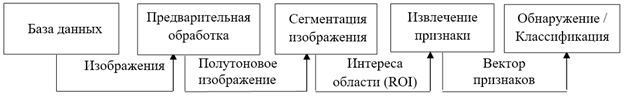
\includegraphics[width=1\linewidth]{pic14}
\caption{Основные этапы системы обнаружения и классификация на основе методов машинного обучения}
	\label{pic14}
	\end{figure}

\textbf{1. Предварительная обработка изображений и извлечение признаков в системах ОКДПП и ОКФП}

Процесс обработки изображений составляет основу разработанных систем так как они должны иметь возможность работать с различным разрешением исходных изображений и работать в режиме времени близкого к реальному. Поэтому процесс обработки изображений должен быть изучен и оптимизирован для того, чтобы система производила качественные результаты, но обеспечивала высокую производительность системы. Этот процесс включает в себя фильтрацию шума и получение качественного изображения, выявление признаков объектов на изображении, преобразование изображения в полутоновое изображение, условия освещения могут изменять различные области изображения, что приводит к их деградации. Эти проблемы решаются с помощью адаптивной балансировки гистограмм, также используется авторский метод на основе математической морфологии для повышения качества анализируемых изображений.

\textbf{2. Математическое моделирование и численные методы для сегментации изображений}

Рассмотрим изображение $Y$ размера $M \times N$. $S = \left\{s\right\}$ - это множество всех расположений пикселя, $s \left(i, j\right)$ - позиция пикселя. Для каждого расположения $s$ существует значение $x_s=\left\{0;1\right\}$, которое определяет состояние пикселя в позиции $s$ какой-то области. Результатом сегментации являются наборы ROI: $\bigcup\ s_{i,j} | x_{s_{i,j}}=1$.

\textit{2.1 Численные методы для сегментации изображений в системе ОКДДП.} В настоящем исследовании метод разрезов на графах применен для решения задач сегментации изображений которые имеют сложную структуру на основе анализа соотношения компонентной связности между пикселами для построения карты дефектов. Построение карты дефектов дорожного покрытия -- суть маркировка пикселей на изображении значением (0 - не дефектом; 1-пиксельный дефект) и выполняется в 3 шага:

--\textit{Шаг 1}. Используя метод разреза на графах изображение сегментируется и извлекается область интереса (region of interest -- ROI).

--\textit{Шаг 2}. Результат сегментации дефектов в ROI улучшается с использованием модели марковских случайных полей.

--\textit{Шаг 3}. Построение полной карты дефектов путем сравнения и замены пиксельных меток, которые получены из шагов 1 и 2.


\textit{2.2. Численные методы для сегментации изображений в системе ОКФП.} Процесс извлечения признаков объектов в изображениях на основе вейвлет-преобразования Хаара выполняется алгоритмом \ref{alg5}.%Пусть графа $ G = \left\{V, E \right\} $ строится узлами $ V $ и ребрами $ E $. Рассмотрены пиксели изображения как узлы, два дополнительных узла $ S $ (источник) для объектов-пучков и $ T $ (терминал) для фона. Для построения взвешенного графа из изображения (рассматривается система $ d = \left(4,8 \right) $ - окрестности). Для каждой пары узлов - это ребра. Функция веса присваивается каждой ребры $ \left (B_ {p, q} \right) $ и приведится ниже.
%
%\begin{equation} \label{eq9}
%B_{p,q}= \exp - \frac{\left(I_p - I_q\right)}{2\sigma^2} \frac{1}{dist\left(p,q\right)}
%\end{equation}
%
%Где $ B_ {p, q} $ - измерение сходства интенсивностей изображения в пикселях $ p $ и $ q $.
%
%
%Область сегментации определяет инициализированные регионы на основе выбранных гистограмм.
%
%
%\begin{equation} \label{eq10}
%\left\{\begin{array}{l} W_p\left('FG'\right)=-\ln His\left(I_p|O\right),\\
%W_p\left('BG'\right)=-\ln His\left(I_p|B\right),
%\end{array}\right.
%\end{equation}
%
%Где $ His \ left (I_p | O \ right) $, $ His \ left (I_p | B \ right) $ - гистограммы интенсивности объекта и фона соответственно.

\begin{algorithm}[ht!]
  \KwData{N изображений.}
  \KwResult{Значения вейвлет-преобразования Хаара (коэффициенты)}
		1. Преобразование изображения RGB в полутоновое изображение;

		2. Изменить размер изображения на ($128 \times 128$);

		3. Предварительная обработка (фильтрация шума, морфологическая обработка)

		4. Вейвлет-преобразование для создания вектора $\vec{I_i}, i=1..N$;

		5. Среднее значение: $I_N=\frac{1}{N}\sum_{i=1}^N I_i$

		6. Расчет для каждого объекта: $\vec{u_i}=\sum_{k=1}^N V_{ik} \phi_k, i=1..N$\\
		$\phi_k=\vec{I_i}-\vec{I_N}$: вычитание среднего изображения из каждого изображения.
			$V_{ik}$: вектор каждой матрицы $W^tW, W=\left\{\vec{\phi_1},...,\vec{\phi_N}\right\} $
  \caption{Извлечение признаков пузырей вейвлет-преобразованием Хаара}\label{alg5}
\end{algorithm}

Для сравнения полученных значений вейвлет-преобразования Хаара используется универсальный порог $ T = \sigma \sqrt {2 \ln n} $, где $ \sigma $ - среднее абсолютное отклонение, а $ n $ - количество выборок конкретных коэффициентов вейвлет-преобразования. Частота дискретизации и масштаб вейвлет-разложения фиксированы $ T = k \sigma $, где $ k = \sqrt {2 \ln n} $ является параметром.

\textbf{3. Математическое моделирование для классификации объектов в системе ОКДДП}

Пусть $S=\left\{X, Y\right\}$ - множество N обучающих выборок, набор дефектов дорожного покрытия признаков $X=\left\{x_i | i = 1, ..., 5\right\}$ и набор меток классов $Y = \left\{y_i |i = 1, ..., 3\right\}$. Классификатор - это функция $H: X \rightarrow Y$, которая отображает $x$ в элемент $y$ из $Y$. Это значит, построение модели обучения и тестирования для классификации объектов по меткам $Y$.

Используется алгоритм случайного леса для классификации дефектов: сети трещин, глубоких трещин и выбоин. Таким образом, каждое дерево строится на множестве $N_t$, это множество случайным образом выводится из $N$. Данные обучения $N_p$ узла $p$ делятся на два набора: $N_l$ - слева и $N_r$ – справа должны следовать пороговое значение $c$ характеристического вектора $v$ в функции $f$:
\begin{equation}\label{eq11}
N_l = \left\{n \in N_p | f\left(v_n\right) > c\right\};  \\
N_r=N_p / N_l.
\end{equation}
На каждом узле создается группа $ m $ -функции, которая случайным образом предлагается для функции $ f $ и находит все возможные значения $ c $ и выбирает из них значение. Чтобы получить самый высокий индекс Джини:
\begin{equation}\label{eq12}
\Delta I_G\left(N_p\right)=I_G\left(N_p\right) - \frac{|N_l|}{|N_p|}I_G\left(N_l\right) - \frac{|N_r|}{|N_p|}I_G\left(N_r\right),
\end{equation} где $I_G\left(N\right)$ - индекс Джини \footnote {Louppe, Gilles and Wehenkel, Louis and Sutera, Antonio, Understanding Variable Importances in Forests of Randomized Trees, Proceedings of the 26th International Conference on Neural Information Processing Systems, Curran Associates Inc., USA, V. 1, N. 9, P. 431--439, 2013} для данных изучения $N$.

\newpage \textbf{Численный метод для классификации на основе алгоритма случайного леса}.

Численный метод основан на алгоритме случайного леса (алгоритм \ref{alg4}) для решения проблемы классификации дефектов дорожных покрытий в системе ОКДДП.
\begin{algorithm}[ht!]
  \KwData{$T$ - количество деревьев; $N$ - количество выборок из набора данных.}
  \KwResult{$y\left(x_i\right)$ - метка для объекта}
   1. \For{\texttt{$t := 1$ to $T$ }}
     {
		1.1 Создавать $M$ - новый шаблон данных с $n$ - размер $M$ из исходного набора данных $N$;

		1.2 Создавать дерево классификаторов для каждого$M$;

		1.3 \For{\texttt{$i := 1$ ко всем узлам}}
     {
		  1.3.1 Получить случайные  $mtry$ признаки из оригинальной функции;

			1.3.2. Выбор лучшего раскола в $mtry$ признаке;
		}
		1.4 $y\left(x_t\right)$ = метка $t$ дерева;
		}

		2. Вернуть $y\left(x_i\right)$ = $\left\{y\left(x_t\right)\right\}^T$ - большинство голосов;

  \caption{Классификация объектов на основе алгоритма случайного леса}\label{alg4}

\end{algorithm}

В данном разделе описывается классификация, основанная на методе обучения с учителем (рис. \ref{pic26}) -- алгоритм случайного леса в дальнейшем принимает концепцию дерева решений, производя большое количество деревьев решений. Сначала извлекается случайная выборка данных и определяется ключевой набор признаков, чтобы вырастить каждое дерево решений. Эти деревья решений, то есть их «Out-Of-Bag» определяют ошибку (частота ошибок модели), а затем ряд деревьев решений сравнивается, чтобы найти совместный набор переменных, которые производят самую точную модель классификации.

\begin{figure}[ht!]
\centering
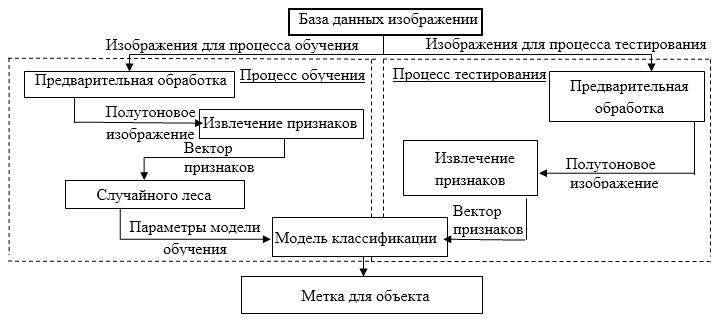
\includegraphics[width=1\linewidth]{pic26}
\caption{Блок схема классификации объектов в системе ОКДДП}
	\label{pic26}
		\end{figure}

В \textbf {третьей главе} дается описание реализации алгоритмов и методов машинного обучения для построения систем ОКДДП и ОКФП для которых в главе 2 были разработаны соответствующие математические модели. Описана структура программ ОКДДП (рис. \ref{pic47}) и ОКФП (рис. \ref{pic59}) и приведены результаты экспериментов для оценки разработанного метода обнаружения и классификации данных на изображении. Проанализирована эффективность предлагаемого метода в сравнении с другими передовыми методами.
\begin{figure}[ht!]
\centering
\vspace{-0.8em}
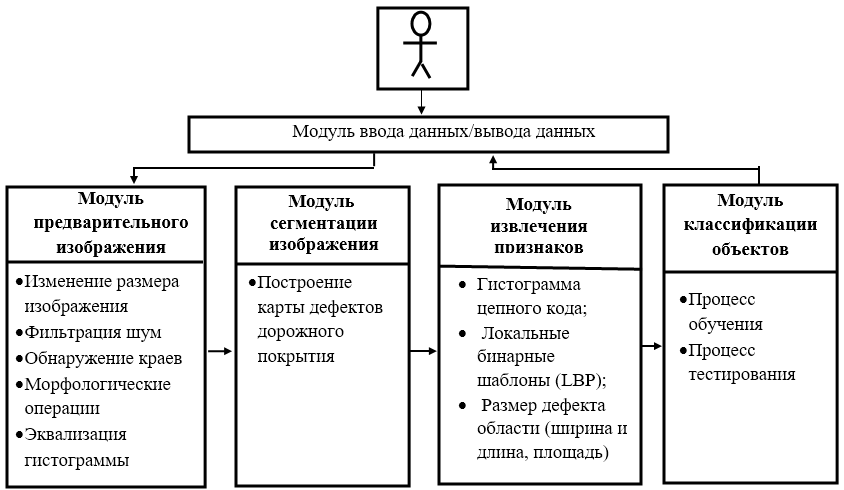
\includegraphics [width=1\linewidth]{images/pic47.png}
%\captionsetup{justification=justified, labelsep=period}
\caption{Структура ПО системы ОКДДП} \label{pic47}
\end{figure}

\begin{figure}[ht!]
\centering
\vspace{-0.8em}
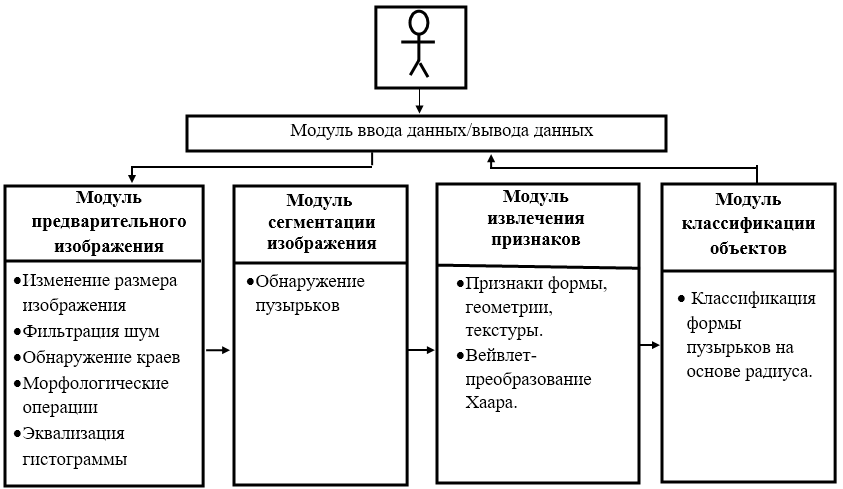
\includegraphics [width=1\linewidth]{images/pic59.png}
%\captionsetup{justification=justified, labelsep=period}
\caption{Структура ПО системы ОКФП} \label{pic59}
\end{figure}

Проведены эксперименты по классификации дефектов дорожного покрытия. Эти эксперименты показали (рис. \ref{pic1}), что предлагаемые алгоритмы обладают, с высокой эффективностью в том числе на изображениях с шумом и ограниченным освещением, что особенно важно для их практического использования. Результаты экспериментов продемонстировали эффективность классификации различных типов дефектов. Сравнение полученных результатов с результатами приложения с других алгоритмов машинного обучения подтвердило стабильность системы, точность и приемлемое время выполнения.
\begin{figure}[ht!]
\centering
\vspace{-0.8em}
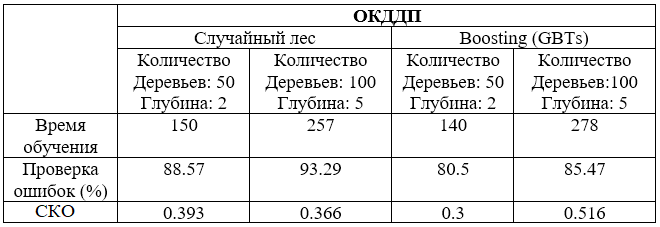
\includegraphics [width=1\linewidth]{images/pic1.png}
%\captionsetup{justification=justified, labelsep=period}
\caption{Время обучения, истинная скорость и проверка ошибок алгоритмов классификации} \label{pic1}
\vspace{-0.8em}
\end{figure}

В \textbf{четвертой главе} представлены инструменты для разработки систем распознавания и классификации объектов: язык программирования Matlab и библиотека OPENCV с открытым исходным кодом. Предоставляются инструкции для пользователей программ. Представление интерфейса и основных функций системы обнаружения и классификации дефектов дорожного покрытия включают в себя следующие функции: ввод данных, предварительная обработка изображений, сегментация изображения и построение карты дефектов дорожного покрытия, извлечение признаков, классификация типов дефекты. Дано описание интерфейса и основных функций системы для обнаружения и классификации форм пузырьков: ввод данных, предварительная обработка изображений, сегментация изображения и обнаружение пузырьков, извлечение признаков, классификация формы пузырьков. Программный модуль имеет простой, удобный и интуитивно понятный интерфейс.

 \textbf{
\begin{center}
ОСНОВНЫЕ РЕЗУЛЬТАТЫ ДИССЕРТАЦИОННОЙ РАБОТЫ
\end{center}
}

1.	Предложены и разработаны математическая модель и численный метод на основе комбинации алгоритмов разреза на графах и Марковского случайного поля для сегментации изображений для построения карты дефектов дорожного покрытия в системе ОКДДП; использована комбинация метода разреза на графах с вейвлет-преобразованием Хаара для обнаружения пузырьков в системе ОКФП.

2.	Проведен анализ и извлечение соответствующих признаков для разных объектов в каждой системе, особое внимание уделено признаку текстуры, геометрическому признаку  и вейвлет-преобразованию.

3.	Разработан метод машинного обучения на основе алгоритма случайного леса для разработки модели классификации объектов в системах ОКДДП и ОКФП.

4.	На основе экспериментов проведен анализ и сравнение фактических результатов обнаружения и классификации дефектов дорожного покрытия в системе ОКДДП; обнаружения и классификации формы пузырьков в системе ОКФП. Результаты эксперимента показывают, что алгоритмы работают на высокой скорости, точности и стабильности системы, обеспечивая работу с шумом и в режиме реального времени.

5.	Созданы программные модули ОКДДП и ОКФП, которые используются для обнаружения и классификации объектов на изображениях в режиме реального времени.

\newpage \textbf{\begin{center}СПИСОК ОСНОВНЫХ РАБОТ ПО ТЕМЕ ДИССЕРТАЦИИ\end{center}}

\hspace{-1.5cm}\textbf{Издания, входящие в Перечень ВАК РФ}

1. \textbf{Нгуен Т.Х.} О распознавании и классификации дефектов дорожного покрытия на основе изображений / Т. Х. Нгуен, Т. Л. Нгуен // Вестник Иркутского гос. технического ун-та. -- 2016. -- №~10 (117). -- С. 111--118.

2. \textbf{Nguyen T.H.} A Robust Approach for Defects Road Pavement Detection and Classification / D. N. Sidorov, T. H. Nguyen, T. L. Nguyen // Journal of Computational and Engineering Mathematics. -- 2016. -- V. 3. -- No. 3. -- P. 40--52.

3. \textbf{Nguyen T.H.} On Road Defects Detection and Classification / T. H. Nguyen, T. L. Nguyen, A. Zhukov // CEUR Workshop Proceedings. -- 2016. -- V. 1710, -- P. 266--278.

4. \textbf{Nguyen T.H.} Machine learning algorithms application to road defects classification / T. H. Nguyen, T. L. Nguyen, D. N. Sidorov, A. I. Dreglea // Intelligent Decision Technologies. -- 2017. -- V. Preprint. -- No. Preprint. -- P. 1--8.

5. \textbf{Nguyen T.H.} Robust Approach to Detection of Bubbles Based on Images Analysis / T. H. Nguyen, T. L. Nguyen, A. I. Dreglea // International Journal of Artificial Intelligence. -- 2018. -- V. 16. -- No. 1. -- P. 167--177.

6. \textbf{Нгуен Т.Х.} Об автоматизации извлечения и классификации антропометрических признаков / Т. Л. Нгуен, Т. Х. Нгуен // Вестник Иркутского гос. технического ун-та. -- 2015. -- №~4 (99). -- С. 17--23.

7. \textbf{Nguyen T.H.} Studies of Anthropometrical Features using Machine Learning Approach / T. L. Nguyen, T. H. Nguyen, A. Zhukov // CEUR Workshop Proceedings. -- 2015. -- V. 1452. -- P. 96--105.

8. \textbf{Nguyen T.H.} Automatic Anthropometric System Development Using Machine Learning / T. L. Nguyen, T. H. Nguyen // BRAIN. Broad Research in Artificial Intelligence and Neuroscience. -- 2016. -- V. 7. -- P. 5--15.

 \newpage \hspace{-1.5cm}\textbf{Свидетельства о государственной регистрации программы для ЭВМ}

9. \textbf{Нгуен Т.Х.} Обнаружение и классификация пузырьков на цифровых изображениях / Д. Н. Сидоров, Т. Х. Нгуен, Т. Л. Нгуен // Свидетельство о гос. регистрации программы для ЭВМ. № 2018612096 от 12 февраля 2018 г. М.: Федеральная служба по интеллектуальной собственности. 2018.

10. \textbf{Нгуен Т.Х.} Программа автоматического обнаружения и классификации дефектов дорожного покрытия / Д. Н. Сидоров, Т. Х. Нгуен, Т. Л. Нгуен // Свидетельство о гос. регистрации программы для ЭВМ. № 2016619386 от 18 августа 2016 г. М.: Федеральная служба по интеллектуальной собственности. 2016.

11. \textbf{Нгуен Т.Х.} Программа бесконтактной антропометрии для смартфонов на операционной системе Андроид / Д. Н. Сидоров, Т. Л. Нгуен, Т. Х. Нгуен // Свидетельство о гос. регистрации программы для ЭВМ. № 2016611475 от 03 февраля 2016 г. М.: Федеральная служба по интеллектуальной собственности. 2016.

	\hspace{-1.5cm}\textbf{Прочие издания}

12. \textbf{Нгуен Т.Х.} Автоматизация антропометрических измерений и извлечение признаков из 2D-изображений / Т. Л. Нгуен, Т. Х. Нгуен // XVI Байкальская международная школа-семинар <<методы оптимизации и их приложения>>. О. Ольхон, Иркутск 2014г. -- С. 153.

13. \textbf{Нгуен Т.Х.} Построение программы для обнаружения контуров человека в изображении с помощью методов математической морфологии / Т. Л. Нгуен, Т. Х. Нгуен // Материалы всероссийской молодежной научно-практической конференции <<Винеровские чтения 2014>>. Иркутск: Изд-во Иркутск, 2014. -- С. 10.

14. \textbf{Нгуен Т.Х.} Классификация и кластерный анализ антропометрических признаков / Т. Л. Нгуен // Материалы всероссийской молодежной научно-практической конференции <<Винеровские чтения 2015>>. Иркутск: Изд-во Иркутск, 2015. -- С. 8.

15. \textbf{Нгуен Т.Х.} Методы математической морфологии в цифровой обработке изображений / Т. Л. Нгуен, Т. Х. Нгуен // Труды XIX Байкальской Всероссийской конференции <<информационные и математические технологии в науке и управлении>>. Иркутск: ИСЭМ СО РАН, 2014. -- С. 75--81.

16. \textbf{Нгуен Т.Х.} Анализ антропометрических признаков с использованием методов машинного обучения / Т. Л. Нгуен, Т. Х. Нгуен // Междисцплинарные исследования в области математического моделирования и информатики . Ульяновск: Изд-во SIMJET, 2015. -- С. 204--210.

\begin{center}
\vspace{0.6cm}
Подписано в печать XX.XX.2018. Формат 60 x 90 / 16.\\
Бумага офсетная. Печать цифровая. Усл. печ. л. 1,25.\\
Тираж 100 экз. Заказ XXX. Поз. плана 10н.\\
\vspace{0.6cm}
Отпечатано в типографии Издательства\\
ФГБОУ ВО «Иркутский национальный\\
исследовательский технический университет»\\
664074, г. Иркутск, ул. Лермонтова, 83.
\end{center}
\thispagestyle{empty}
